\section{Universal Second Factor}

The \glsfirst{u2f} is the second open standard developed by the \gls{fido} alliance prior to the \wa. It explicitly defines a second factor for the password-based login flow. It is like the \gls{uaf} backed by public-key cryptography, too. The main contributors are Google and Yubico, both being alliance members. The \textit{strong second factor} can be either connected or disconnected, e.g, built in hardware orl for instance, an \gls{usb} token, \gls{nfc}-capable device, or a standalone \gls{ble} dongle. Besides that, the \gls{u2f} protocol only specifies \gls{usb}-\gls{hid} devices (internal or external), \gls{nfc}, Bluetooth, and the low energy variant \gls{ble}, as possible transport protocols. The protocol defines two layers:\footcites[See][4]{u2f-overview}[See][4]{u2f-js-api}

\begin{enumerate}
	\item the first layer defines the cryptographic basics of the protocol
	\item the second layer defines the communication between the user's authenticator and the first layer over the chosen transport protocol (such as \gls{usb}, \gls{nfc}, or \gls{ble})
\end{enumerate}

The \gls{u2f} protocol relies on a web browser that is \gls{u2f}-capable, a web server that supports \gls{u2f} protocol, and the authenticator, called the \gls{u2f} token. Two different operations are defined by the specification, the \textit{registration} and \textit{authentication}. Authentication is performed by generating a signature. A notable difference to the \gls{uaf} protocol is the absence of a de-registration request. The message frame defined by the standard is based on the \gls{iso} standard for smartcards (ISO-7816) \gls{apdu}.\footcites[See][3]{7860546}[See][3]{u2f-raw-message}

Because \gls{u2f} relies on the web in contrast to the \gls{uaf} protocol, browser support has to be taken into account. Due to the fact, that \gls{u2f} is superseded by \gls{fido}2, the browser support of \gls{u2f} is not of interest for this thesis.

Moreover, \gls{u2f} has been renamed to \gls{ctap}-1 since the release of \gls{fido}2 to avoid confusion and questions whether \gls{u2f} as the \gls{ctap} can be used for the \wa.\footcite[See][4]{ctap2}

\subsubsection{Registration}

\begin{figure}[hbt]
	\centering
	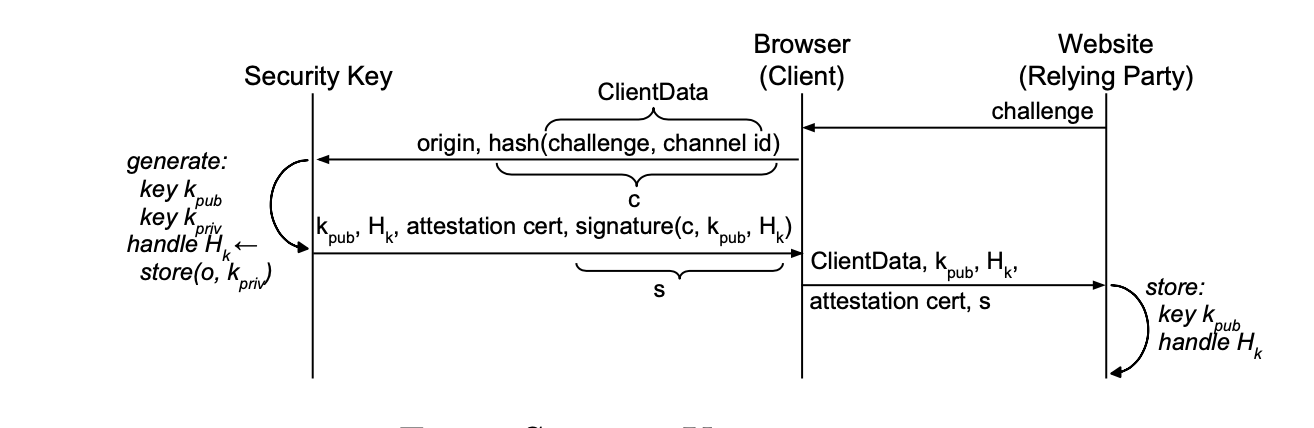
\includegraphics[width=\textwidth]{pics/u2f_reg}
	\caption[\gls{u2f} registration process]{\gls{u2f} registration process\footnotemark}
	\label{fig:u2f_reg}
\end{figure}
\footcitetexts[Source: diagram by author, based on][69]{10.1007/978-3-319-75650-9_5}[][428]{10.1007/978-3-662-54970-4_25}

A requirement of the registration process of a \gls{u2f} token is that the user already is registered on the \gls{rp}, the web server. The registration process is similar to the introduced process of the \gls{uaf} protocol and also displayed in \autoref{fig:u2f_reg}. At first, the server generates a \textit{challenge} for the client and sends it along with the \textit{username} and its \textit{AppID} to the client, in this case the web browser. The payload also contains the desired \textit{version} of the \gls{u2f} protocol and the already \textit{registered keys}, if any. The client can verify that the AppID matches the origin it is communicating with.\footcites[See][4--5]{u2f-js-api}[See][431]{10.1007/978-3-662-54970-4_25}

Further, the challenge parameters are constructed by hashing \textit{client data}, i.e., the challenge, AppID, and \textit{typ}. The typ always has the value \textit{navigator.id.finishEnrollment} for a registration process. This data along with the hash of the AppID is sent to the \gls{u2f} token. After that, the token optionally verifies the presence of the user and generates a new key-pair over the \gls{nist} \gls{ec} P-256 and stores it with the username in its database. The token sends the \textit{registration data} consisting of the public key, i.e. an uncompressed point on an \gls{ec} and the key handle, which can be wrapped, i.e., encrypted, back to the client. In addition, the attestation certificate of the token and an \gls{ecdsa} signature over the hashed AppID, hashed challenge, key handle, and public key are sent back to the client.\footcites[See][4--5]{u2f-raw-message}[See][70]{10.1007/978-3-319-75650-9_5}

Finally, the client forwards the registration and client data to the \gls{rp}, which can cryptographically verify the data with the signature and attestation certificate.\footcites[See][3]{7860546}

The following \autoref{listing:u2freg} shows the high-level \gls{js} \gls{api} registration process.
\\
\begin{example}{Example U2F registration request}{listing:u2freg}
\begin{minted}[breaklines]{javascript}
const registerRequest = {
  challenge: 'Wings2019', // usually a random string
  version: 'U2F_V2' // where V2 refers to protocol version 1.2
  appId: 'https://timbrust.de'
};

const registeredKeys = [];

u2f.register('https://timbrust.de', [registerRequest], registeredKeys, (response) => {
  console.log(response)
});
\end{minted}
\end{example}

The challenge value in the \textit{registerRequest} usually is a random challenge and base64 encoded, but for demonstration purposes a plain text string is used instead. In a real world scenario, the \textit{registerRequest} object is generated by the \gls{rp} and sent to the client and the \textit{u2f} \gls{js} object is called by the client. Passing in a list of already registered keys with the \gls{rp} avoids the duplicate registration of a user with the \gls{rp}.\footcites[See][3]{u2f-js-api}[See][430]{10.1007/978-3-662-54970-4_25}

The received response is displayed in \autoref{listing:u2fregresp} and contains the already explained \textit{registrationData} and \textit{clientData}, both being  the base64 encoded. For better readability the strings clientData and registrationData are trimmed. Also, the clientData is decoded to show which data it contains. The client always returns an \textit{errorCode} OK (0) indicating a successful registration. Other error codes include a bad request (2), unsupported configuration (3), ineligible device (4), timeout (5), or an other error (1). Further the clientData consists of \textit{typ}, as well as the challenge of the \gls{rp} and the origin.\footcites[See][7]{u2f-js-api}[See][8]{u2f-raw-message}

\begin{example}{Example U2F registration response}{listing:u2fregresp}
\begin{minted}[breaklines]{javascript}
const response = {
  clientData: 'eyJjaGFsbGVuZ2UiOiJXaW5nczIwMTkiLCJvcmlnaW4i [...]', // further data is omitted for readability
  errorCode: 0,
  registrationData: '...', // omitted for readability
  version: 'U2F_V2'
};

// btoa() decoded clientData yields
const decodedClientData = {
  challenge: 'Wings2019',
  origin: 'https://timbrust.de',
  typ: 'navigator.id.finishEnrollment'
};
\end{minted}
\end{example}

\subsubsection{Authentication}

The authentication process involves signing a challenge from \gls{rp} with the corresponding private key. This enables the \gls{rp} to cryptographically verify the the response with the saved public key. \autoref{fig:u2f_auth} shows the procedure, too. The \gls{rp} begins by sending a random \textit{challenge}, the \textit{key handle} associated with the user, and the \textit{AppID} to the client. As in the registration phase, the client can verify the received AppID to the origin it communicates with.\footcites[See][3]{7860546}[See][6]{u2f-js-api}

Afterwards, the challenge parameters are constructed by hashing the challenge, AppID, and \textit{typ}. The typ is always set to \textit{navigator.id.getAssertion} for an authentication. This data is sent along with the hashed AppID to the \gls{u2f} token. There is no difference in this process compared to the registration.\footcites[See][6]{u2f-raw-message}

Upon reception, the \gls{u2f} token verifies the presence of the user and retrieves the stored key-pair associated with the key handle. It sends the counter, that is increased by each usage, and the \gls{ecdsa} signature over the values user presence, counter, challenge parameters and the hashed AppID back to the client.\footcites[431]{10.1007/978-3-662-54970-4_25}[See][7]{u2f-raw-message}

The client forwards registration data, client data, and key handle to the \gls{rp}, which in return can verify the signature data with the stored public key.\footcites[See][118]{IdentityandDataSecurityforWebDevelopment}

\begin{figure}[hbt]
	\centering
	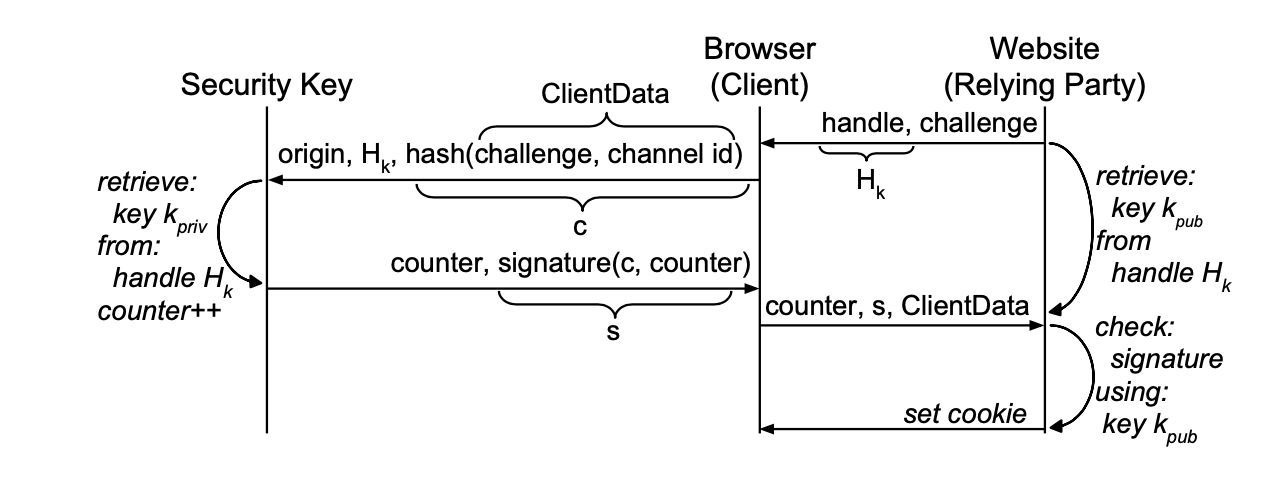
\includegraphics[width=\textwidth]{pics/u2f_auth}
	\caption[\gls{u2f} authentication process]{\gls{u2f} authentication process\footnotemark}
	\label{fig:u2f_auth}
\end{figure}
\footcitetexts[Source: diagram by author, based on][70]{10.1007/978-3-319-75650-9_5}[][428]{10.1007/978-3-662-54970-4_25}

The \autoref{listing:u2fauth} shows an example, high-level \gls{js} \gls{api} signing process. The \gls{rp} sends the associated key handle, the protocol version, AppID and authentication challenge to the client. \autoref{listing:u2fauthresp} shows the generated response by the \gls{u2f} token. The response object and decoded client data shows the \autoref{listing:u2fauthresp}, where the clientData can also be generated beforehand by the client.\footcites[See][3]{u2f-js-api}
\\
\begin{example}{Example U2F authentication request}{listing:u2fauth}
\begin{minted}[breaklines]{javascript}
const registeredKey = {
  keyHandle: '_WFf5BJ1dwtSCFzfWHoqKUhc9M3Hi0Tv58LAtPz0qM6B3A [...]', // further data is omitted for readability
  version: 'U2F_V2'
};

u2f.sign('https://timbrust.de', 'Wings2019Auth', [registeredKey], (response) => {
    console.log(response)
  }
);
\end{minted}
\end{example}

\begin{example}{Example U2F authentication response}{listing:u2fauthresp}
\begin{minted}[breaklines]{javascript}
const response = {
  clientData: 'eyJjaGFsbGVuZ2UiOiJXaW5nczIwMTlBdXRoIiwib3JpZ2H [...]', // further data is omitted for readability
  errorCode: 0,
  keyHandle: 'WFf5BJ1dwtSCFzfWHoqKUhc9M3Hi0Tv58LAtPz0qM6B3A-iT [...]', // further data is omitted for readability
  signatureData: 'AQAAAhIwRQIhAK7xli8pV2cc8TKTOYMcdiz-ZuNVes [...]', // further data is omitted for readability
};

// btoa() decoded clientData yields
const decodedClientData = {
  challenge: 'Wings2019Auth',
  origin: 'https://timbrust.de',
  typ: 'navigator.id.getAssertion'
};
\end{minted}
\end{example}

The client forwards the response to the \gls{rp}. It consists of the client data, not its hash, the error status, as well as the key handle and the signature data, signed with the private key.